Gaussian distribution, also known as \textbf{normal distribution}, is represedted by the following \textbf{Probability Density Function}:

\begin{listequbox}
  {\text{PDF}_{\mu\text{,}\sigma}(x) = \dfrac{1}{\sigma\sqrt{2\pi}} e^{-\dfrac{(x-\mu)^2}{2\sigma^2}}}{equgaussdst}{Probability density function}
\end{listequbox}

where $\mu$ is the mean and $\sigma$ is the standard deviation of a very large data set. The Gaussian distribution is a bell-shaped curve, symmetric about the mean value. Probability density functions represent the spread of a data set. An example is shown below.

\begin{grafica}[H]
\center
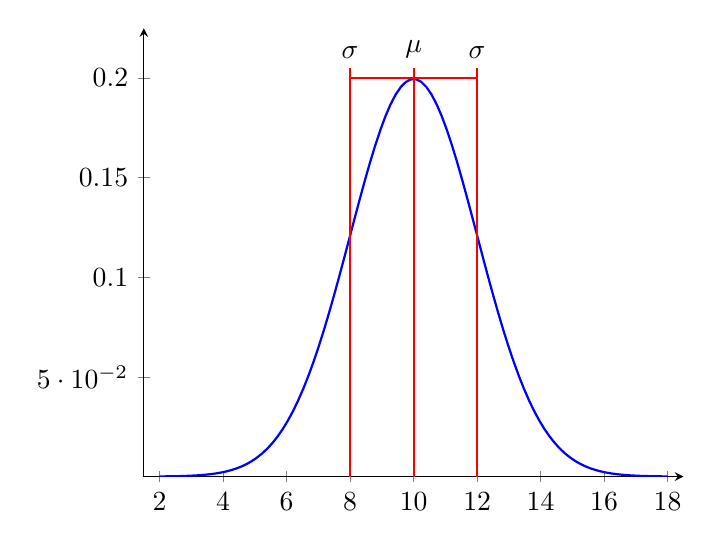
\begin{tikzpicture}
  \begin{axis}[
    xmin=1.5,xmax=18.5,
    ymin=0,ymax=0.225,
    axis lines=center
    ]
    \addplot[color=blue,samples=100,domain=2:18,thick]{(1/(2*sqrt(2*pi)))*exp(-((x-10)^2)/(2*(2^2)))};

    \draw[red,thick] (axis cs:8,0) -- (axis cs:8,0.205);
    \draw[red,thick] (axis cs:10,0) -- (axis cs:10,0.205);
    \draw[red,thick] (axis cs:12,0) -- (axis cs:12,0.205);
    \draw[red,thick] (axis cs:8,0.2) -- (axis cs:12,0.2);

    \node[above] at (axis cs:8,0.205) {$\sigma$};
    \node[above] at (axis cs:10,0.205) {$\mu$};
    \node[above] at (axis cs:12,0.205) {$\sigma$};
  \end{axis}
\end{tikzpicture}
\caption{Gaussian distribution}
\end{grafica}

In this specific example, $\mu$ = 10 and $\sigma$ = 2.

Normal distribution is completely defined by the mean ($\mu$) ans the standard deviation ($\sigma$). The line never touches the x-axis. The y-axis acts as the probability. Total area under curve is 1, because the sum of all probabilities is 1.
